\documentclass{report}
\usepackage{graphicx} % Required for inserting images
\usepackage{makeidx}
\usepackage{setspace}
\usepackage{authblk}
\usepackage{pdfpages}


\usepackage[margin=1.2in]{geometry}
\usepackage{geometry}

\title{Rastreamento e Monitorização da Execução de Programas\\
\Large Universidade do Minho}

\author{João Luís da Cruz Pereira (a95375) \and
Maria Helena Alves Machado Marques Salazar (a75635) \and
Miguel António Vaz Pinto Pereira (a72161)\\}
\date{April, May 2023}

\begin{document}
\spacing{1.25}

\maketitle
\tableofcontents
\newpage
\section{Introdução}
Através deste projeto, pretendemos implementar um serviço de monitorização eficaz de um ou vários programas.\\

A monitorização e rastreio da execução de programas são aspetos críticos do desenvolvimento e manutenção de software, que consistem na observação do comportamento do programa para identificar erros, problemas de desempenho, entre outros. Uma das formas eficazes de rastrear a execução de programas é através de chamadas de sistema, que possibilitam ao programa solicitar serviços ao \textbf{kernel} do sistema operacional e interagir com o sistema operativo subjacente de forma segura e padronizada.\\

Neste projeto serão utilizados serão usados pipes e \textbf{FIFOS} (pipes com nome) para implementar uma variedade de funcionalidades que permitem o fluxo de dados entre diferentes processos num sistema operativo, permitindo uma comunicação eficiente e em tempo real entre programas. No caso deste projeto, esta comunicação será vital para o bom funcionamento entre o cliente e o servidor, bem como entre os vários processos filhos a executar \textit{(por vezes, em simultâneo)}.\\

O objetivo deste projeto é concretizar uma comunicação sólida e segura entre um possível cliente e servidor, usando pipes, chamadas de sistema e uma variedade de outras técnicas para monitorizar, rastrear e guardar a informação relativa ao programas em execução.\par 
Espera-se que no término do desenvolvimento feito pelo grupo, todas as funcionalidades \textit{(básicas e avançadas)} estejam corretamente implementadas e toda a conexão esteja operacional e segura.

\newpage
\section{Funcionalidades Básicas}
\subsection{Execução de programas por parte do utilizador}

Em \textbf{geral,}\\

Para prosseguir com a execução do programa em questão, definiu-se uma função execute onde se processa a inicialização com um \textbf{fork} \textit{(para permitir a execução sem um término prévio do programa)} e o comando procede com os respectivos argumentos.\par
Foram também escritas mensagens de erro caso aconteçam durante o correr do código, desde a impossibilidade de criação de um processo filho à execução através do \textbf{execvp}.\par
Os argumentos em questão foram separados por uma função tokenizer e durante todo o processamento de dados do código será maioritariamente suportado por uma struct prog. Seguem-se então breves explicações sobre a construção e funcionamento destes.

\subsubsection{\underline{Tokenizer}}

Derivado da criação da funcionalidade \textbf{execute -u}, onde será necessário analisar o conteúdo da string fornecida pelo utilizador ao cliente, surgiu a necessidade da criação de um sistema auxiliar que nos permita dividir esta em seus vários componentes \textit{(cujo parâmetro de divisão seja o caracter espaço)}.\\
Com isto em mente, recorreu-se a uma função tokenizer, aonde se dá a separação do input introduzido pelo utilizador em tokens de formato string \textit{(que posteriormente serão armazenados array)}, o que então possibilita o uso do conteúdo do programa em si – o seu comando e respetivos argumentos – em outras funcionalidades do projeto.

\subsubsection{\underline{Struct \textbf{PROG}}}

Para a transição de informação entre o cliente e o servidor de um programa \textit{(entre os pipes e, por continuidade, as pipelines)}, procedeu-se a criação de uma struct que armazena todos os dados aos quais pretendemos trabalhar com; desde o comando em si, argumentos associados, o tempo de iniciação do processo e respetivo tempo de execução. Deste modo, haverá menos perda de informação e esta estará organizada de uma maneira mas sucinta.

\subsubsection{\underline{Novo Programa do Utilizador e Respectiva Terminação}}

\subparagraph{Cliente:}
A funcionalidade básica do projeto, o \textbf{execute}, procede com a cálculo de um processo filho que estará conectado a um pipe que servirá para futuro intercâmbio de informação com os processos a correr. Prossegue-se então para a execução os comandos que serão introduzidos pelo utilizador seguido da função.
Com a função \textbf{gettimeofday}, procedemos a atribuição do tempo inicial ao qual um programa começa a executar e passa-se essa informação através de uma struct previamente criada a fim de guardar o \textbf{PID} \textit{(do filho em causa)} e esse mesmo tempo para o processo pai através de um pipe anónimo e ao servidor atravès de um \textbf{FIFO}.\par
Neste processo, também será enviado o nome do comando que foi executado com sucesso.\\

Assim que o processo filho termina a sua execução, o processo pai (que estava em modo \textbf{WAIT}, ou seja, em modo espera) chama também a função gettimeofday para obter o tempo de término e com a informação recebida do filho, este calcula a diferença entre ambos – isto é, o tempo que o programa demorou a executar. Essa duração em milissegundos juntamente com o \textbf{PID} do processo filho que acabou de concluir serão então enviados para o servidor por \textbf{FIFO}.\\

Durante o correr das introduções deste pedaço de código, o utilizador é informado do \textbf{PID} do programa que está a correr e no final, o tempo de execução do mesmo. O utilizador também é informado de vários erros que posso acontecer durante a execução.

\subsubsection{\underline{Store}}
No seguimento de obtenção de uma melhor dinâmica de consulta de programas ainda em execução \textit{(e suas respectivas informações}, decidiu-se proceder a criação de um array chamado store que armazena em cada posição uma \textbf{struct prog} com esses mesmo dados. Sendo assim, torna-se uma das peças chave no código do projeto.
\subsubsection{\underline{Server Block}}
Para manter o servidor a correr, foi aberto um descritor de escrita que se mantém bloqueado enquanto não houver descritores de leitura abertos, mantendo assim o servidor a correr para "sempre".
\subsection{Kill}
Para evitar possíveis consequências \textit{(como o não fazer unlink e close)} com o fechar do servidor usando o \textbf{CTRL + C}, decidiu-se criar o \textbf{comando kill} para que este ponha um fim ao estado acima definido como \textbf{Server Block}.\\
Este comando interrompe o ciclo de leitura com um break, obrigando o processo a entrar na fase de encerramento dos descritores e unlink dos pipes.

\subparagraph{Servidor:}

Para simplificar o processamento de informação dos vários programas que estão a execução, criou-se um array store que vai armazenar em cada índice struct prog. Tendo este array, inicializamos a leitura do \textbf{PID} enviado e vai consultar se este já existe dentro de algum índice do store. Se encontrado, quer dizer que o programa em questão já terminou; se não encontrar, armazena-o.\\ 

\begin{figure}[b]
    \centering
    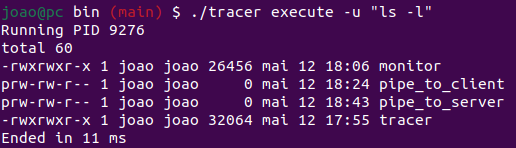
\includegraphics[width = 0.6\textwidth]{figs/execute-u.png}
    \caption{Demonstração da execução do execute-u.}
    \label{f}
\end{figure}

\newpage
\subsection{Consulta dos Programas em Execução}
A função status quais são os programas que estão a executar e o seu tempo até ao momento (milisegundos). Os resultados serão apresentados ao utilizador pelo cliente, listados um por linha.

\subparagraph{Cliente:}

Quando é lido o comando status, abre-se um pipe onde a informação passada por este será feita em \textbf{struct prog}\footnote{Neste caso, decidiu-se comunicar com o servidor pois este está sempre com um processo de leitura direcionado à informação no formato da struct prog.} onde seguirá o comando ‘status’ para o servidor então processar o código associado a esta função. Dado como terminado o reconhecimento dos programas a executar pelo lado do servidor, o cliente lê toda a data enviada e imprime no standard output o \textbf{PID}, o nome do programa e o seu tempo de execução até ao momento.


\subparagraph{Servidor:}

Foi pedido ao servidor o tempo de execução do programa até ao momento e para tal, usa-se a função gettimeofday (como visto previamente). Procedemos com a abertura de um pipe para o cliente onde será enviada a informação pedida pelo mesmo, desta vez só usando \textbf{strings}\footnote{Quando estabelecidas conexões do servidor para o cliente, o pipe não está dependente de structs. Então, com isto em mente, procurou-se usar strings para o envio desta mesma informação pois facilita o processo em causa.}.
Com o array store passado na função, é feito o cálculo dos vários programas armazenados em struct, sendo depois formatado numa string e enviado pelo pipe acima criado. Depois do ciclo ser dado como terminado, o processo é encerrado com o encerramento desse mesmo pipe e o cliente terá acesso a informação pedida, se nenhum erro ocorrer.\\

\begin{figure}[h]
    \centering
    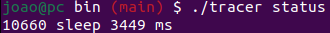
\includegraphics[width = 0.6\textwidth]{figs/status.png}
    \caption{Demonstração da execução do status.}
    \label{f}
\end{figure}

\section{Funcionalidades Avançadas}
\subsection{Execução Encadeada de Programas}

\subparagraph{Cliente:} Inicialmente abre-se um \textbf{FIFO} onde irá ser escrito, tal como no resto das funcionalidades deste programa, uma \textbf{struct prog} que guarda o \textbf{PID} do pipeline \textit{(no caso, \textbf{PID} do processo pai)}, os comandos \textit{(provenientes do utilizador)}, e o ‘start’ \textit{(o valor resultante da função gettimeofday)}. Consecutivamente, envia-se a informação guardada para o servidor pelo pipe. Verificado o envio, o utilizador recebe notificação sobre o ID do processo da pipeline em execução - \textbf{PID} do processo pai.\\

Para executar as funções solicitadas pelo utilizador, o grupo implementou um loop que itera sobre um array de arrays de tamanho dois, onde será criado um pipe em cada posição do arrray usando esse mesmo par. Para uma melhor organização do código, o loop é dividido em três casos distintos.

\subsubsection{\underline{Primeiro Caso}}
No primeiro caso, ou seja, no caso de ser o primeiro programa, é criado um pipe que estabelece comunicação entre este e o segundo programa. Para tal, é necessário alterar o file descriptor 1 para o file descriptor de escrita do pipe, de forma a permitir que o output do primeiro comando seja redirecionado para o próximo pipe em vez de ser escrito diretamente no \textbf{STDOUT}.\par
Após a criação do processo filho, este é responsável pela execução do comando fornecido enquanto o processo pai continua a executar o loop. No entanto, caso ocorra algum erro durante a execução do comando pelo processo filho, a substituição completa do código deste pela chamada ao sistema \textbf{execvp} não ocorrerá, e o programa terminará.

\subsubsection{\underline{Segundo Caso}}
No segundo caso, isto é, no último programa da pipeline, o processo pai criará um novo filho, seguindo um procedimento semelhante ao anteriormente descrito. A diferença reside no facto de que, ao contrário do primeiro caso, o descritor de leitura deve ser alterado em vez do descriptor de escrita, uma vez que o objetivo é ler o output do pipe em vez do \textbf{STDIN}. Para esse fim, a \textbf{função dup2()} é novamente utilizada.\par
Neste caso, é mantido o file descriptor de escrita para o \textbf{STDOUT} pois estamos peranto o último programa a ser executado.

\subsubsection{\underline{Terceiro Caso}}
No terceiro caso, ou seja, para os programas intermédios, é necessário alterar ambos os descritores de ficheiros, uma vez que não se pretende que este pipe leia do \textbf{STDIN} ou escreva no \textbf{STDOUT}, mas sim no descritor de leitura do pipe anterior e no descritor de escrita do pipe atual, respetivamente. Para realizar esta operação, é necessário utilizar a system call \textbf{dup2} duas vezes, para alterar os descritores de ficheiros adequadamente.\\

Deve-se salientar que é necessário fechar os file descriptors que não serão mais utilizados no processo pai. Quando se faz \textbf{fork}, é obtida uma cópia dos mesmos, e se não forem mais utilizados, devem ser fechados para evitar vazamento de memória. O mesmo deve ser feito nos processos filhos, fechando os descritores após o uso, para o bom funcionamento do programa.
Finalmente, o processo pai espera que todos os processos filhos terminem através de um loop de \textbf{wait()}.\par
O código responsável pela execução da pipeline calcula também o tempo de execução total da mesma, utilizando o tempo atual e o tempo inicial armazenado na variável \textbf{start}. A diferença entre ambos é calculada em microssegundos e guardada na \textbf{struct prog}, juntamente com o \textbf{PID} da pipeline. Esta struct é então enviada para o servidor.

\begin{figure}[h]
    \centering
    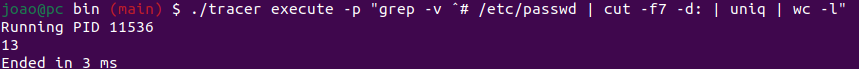
\includegraphics[width = 1\textwidth]{figs/execute-p.png}
    \caption{Demonstração da execução da pipeline.}
    \label{f}
\end{figure}


\subsection{Armazenamento de Informação sobre Programas Terminados}

\subparagraph{Cliente:} Quando o utilizador fornece ao cliente uma das duas opções de execução, este prepara a informação necessária numa \textbf{struct prog} para o servidor avaliar o rumo a tomar. Finalizando o processo, é enviada outra struct com o \textbf{PID} e o tempo de execução.

\subparagraph{Servidor:} Se o servidor não corresponder a nenhuma opção \textit{(status, stats-x e kill)}, então vai usar o PID recebido previamente do cliente para verificar se este é um programa novo ou é um programa que terminou \textit{(através de comparações feitas com as posições do array \textbf{store})}.\par
Tendo o programa encontrado o seu término, é criado um ficheiro na diretoria fornecida pelo utilizador ao executar o monitor. Este ficheiro contém a informçaão fornecida atravès da \textbf{struct}, isto é, os comandos e o tempo de execução e cujo nome é o \textbf{PID} do programa em questão.

\begin{figure}[h]
    \centering
    \includegraphics[width = 0.8\textwidth]{figs/Screenshot20from202023-05-132010-06-44.png}
    \caption{Demonstração da funcionalidade e respetivos ficheiros.}
    \label{f}
\end{figure}

\subsection{Consulta de Programas Terminados}

\subsubsection{\underline{Stats-Time}}
\subparagraph{Cliente:} Na funcionalidade stats-time, o utilizador passa ao cliente uma série de \textbf{PIDs} onde quer que seja calculado o tempo total de execução nos programas dos mesmos.
No lado do cliente é verificado a opção e é passado ao servidor uma struct com o comando \textbf{“stats-time”} e no campo args seguem os \textbf{PIDs} passados pelo utilizador.\par
Todo o processo é efetuado no servidor e no final, o cliente recebe a string previamente formatada através de um \textbf{FIFO}, optando assim por uma solução mais simples em vez de voltar-se a utilizar a struct.

\subparagraph{Servidor:} É enviado ao servidor uma \textbf{struct prog} e essa é lida, entrando na opção stats-time onde a função \textbf{\texttt{status\char`_time}} será chamada para execução. \par
Com isto, percorre-se os \textbf{PIDs} fornecidos, onde segue a abertura do ficheiro correspondente a cada um deles. A leitura é efetuada byte a byte para se conseguir encontrar o final da linha, sabendo assim quando termina o valor em milisegundos do seu tempo de execução \textit{(que se encontra na primeira linha)} e adicionar ao total. Quando a primeira linha termina, o ciclo é interrompido pois já foi obtida a informação pedida.\par
No final de percorrer todos os ficheiros dos \textbf{PIDs}, passa-se o valor total em formato string ao cliente que por sua vez mostra a mesma recebida ao utilizador.

\begin{figure}[h]
    \centering
    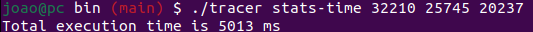
\includegraphics[width = 0.8\textwidth]{figs/stats-time.png}
    \caption{Demonstração da execução da stats-time.}
    \label{f}
\end{figure}

\subsubsection{\underline{Stats-Command}}
A funcionalidade \textbf{stats-command} partilha uma certa similaridade com a funcionalidade \textbf{stats-time}. Porém, a nova recebe mais um argumento para a sua execução proceder conforme o esperado.

\subparagraph{Cliente:}
É passado ao servidor o comando \textbf{stats-command} na \textbf{struct prog} no seu respetivo campo, enquanto que no campo \textit{args}, na primeira posição do array vai o comando a ser procurado enquanto que no resto do array segue os \textbf{PIDs} onde queremos procurar o comando em questão.\par
Terminada a execução por parte do servidor, o cliente recebe uma string formatada para mostrar ao utilizador o resultado pretendido.

\subparagraph{Servidor:}
Recebida a \textbf{struct prog} necessária, este na opção correta e chama a respetiva função. Em seguida, repete-se o processo descrito em cima em relação \textbf{PIDs}, abrindo os respectivos ficheiros. A leitura é na mesma efetuada byte a byte, porém o processo não termina na primeira linha pois é sempre comparado o valor lido nessa linha com o comando pretendido \textit{(na primeira linha lê o valor em milisegundos e compara com o comando na mesma, e certamente que não é obtida nenhuma igualdade)}.\par
Sendo o valor lido equivalente ao comando, é incrementado total o número de vezes quantas aquelas o comando em si é repetido nos \textbf{PIDs} previamente enviados.
Lido o último \textbf{PID}, a informação obtida é então formatada numa string e de novo, através de um \textbf{FIFO} é enviada ao cliente.\\

\begin{figure}[h]
    \centering
    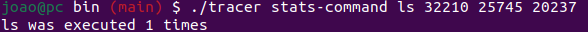
\includegraphics[width = 0.8\textwidth]{figs/stats-command.png}
    \caption{Demonstração da execução da stats-command.}
    \label{f}
\end{figure}

\newpage
\subsubsection{\underline{Status-Uniq}}
No caso do stats-uniq, a similaridade é maior com a primeira funcionalidade descrita na Consulta de Programas Terminados, visto que o campo \textit{args} da \textbf{struct prog} só leva os \textbf{PIDs} e no campo \textit{cmd} leva o \textbf{stats-uniq}.

\subparagraph{Cliente:} Como descrito em cima, é enviado ao servidor uma \textbf{struct prog} com as informações pedidas para o servidor atuar sobre a função definida como \textbf{stats-uniq}.
Visado o término da função no servidor, o cliente recebe as strings dos comandos executados separados por um \textit{\textbackslash n} e apresenta-os ao utilizador.

\subparagraph{Servidor:}
Semelhante as outras duas funções acima descritas, serão percorridos os \textbf{PIDs} fornecidos pelo cliente, abrir os ficheiros correspondentes e verificar os comandos guardados em cada um deles. Com a ajuda de um array \textbf{store}, onde serão armazenados os comandos dos \textbf{PIDs} lidos, serão introduzidos os comandos uma única vez (mesmo havendo repetição). A leitura para obtenção do comando é de novo efetuada byte a byte, ignorando a primeira linha pois esta está reservada para o tempo de execução.\par
No caso de o \textbf{store} estar vazio, adiciona-se imediatamente o comando em questão; senão tem-se que percorrer o array para garantir que esse comando já não está armazenado numa posição.
Com o término da leitura de \textbf{PIDs}, é passado ao cliente os comandos guardados \textit{(depois de convertidos e formatados em string)}, um a um, através de um \textbf{FIFO}. 

\begin{figure}[h]
    \centering
    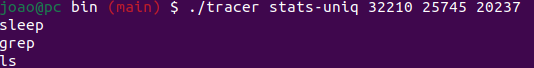
\includegraphics[width = 0.8\textwidth]{figs/stats-uniq.png}
    \caption{Demonstração da execução da stats-uniq.}
    \label{f}
\end{figure}

\newpage
\section{Conclusão}
Com o desenvolvimento do projeto, conseguimos cumprir todas as funcionalidades básicas e avançadas propostas. Segundo os testes que nós efetuamos, não encontramos falhas nas funcionalidades mas as mesmas podem existir de qualquer das formas.\\

Em termos de melhorias possíveis, podiamos tentar com que quando o utilizador por exemplo executa \textbf{./tracer execute -u ls} o programa retornasse erro pois não colocou o programa a executar dentro de aspas. Existe tratamento de erros para quando é colocado \textbf{./tracer execute -u ls -l} devido ao número errado de argumentos mas com o número correeto não.\par
A grande maioria dos problemas que tivemos foi mais com C do que propriamente com a comunicação entre programas/ficheiros, com a exceção de algumas leituras dos pipes que acabaram por ser resolvidas.\\

Foi um trabalho interessante que envolveu toda a matéria usada nas aulas práticas e que apesar de desafiador foi também muito produtivo, pois para além de aprendermos mais sobre a cadeira de \textit{Sistemas Operativos} também aprendemos mais sobre \textit{Git/Github}, \textit{LaTex/Markdown} e mesmo a linguagem \textit{C} em si.


\end{document}
